\documentclass{article}

\usepackage[margin=1in]{geometry}
\usepackage[table]{xcolor}
\usepackage{graphicx}
\usepackage{wrapfig}

\definecolor{lightgray}{gray}{0.8}

\begin{document}

  \title{Homework 1}
  \author{Connor Johnstone}

  \maketitle

  \section{Vostok I}

  \begin{center}
  \rowcolors{1}{lightgray}{white}
    \begin{tabular}{ >{\bfseries}r | p{3.5in} }
      \hline
      Launch Vehicle & Vostok I \\
      Crew & Yuri Gagarin \\
      Dates & 12 April 1961 \\
      Mission Summary & First manned spaceflight \\
      \hline
    \end{tabular}
  \end{center}

  \begin{wrapfigure}{l}{0.25\textwidth}
    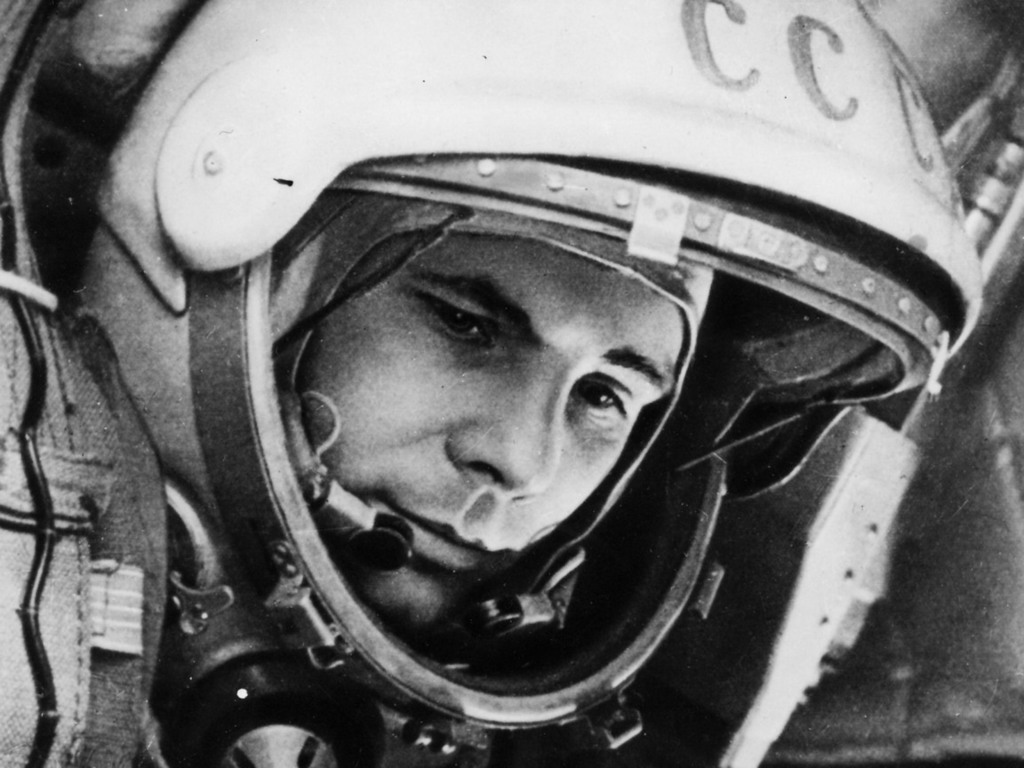
\includegraphics[width=0.9\linewidth]{yuri.jpg}
  \end{wrapfigure}

  While the moon was certainly a new territory, nothing compares to truly
  venturing out into the unknown. Throughout the first week of this class, even,
  we've discussed a wide range of accidental effects and surprises that human
  spaceflight has had in store for us. For a person to take that leap into space,
  knowing that every single effect will be something we, as a human race, will be
  experiencing for the first time and knowing that we couldn't possibly prepare
  for everything that might happen, since we couldn't know everything that might
  happen, is a truly incredible feat of exploration. 
  
  And to top off such an
  accomplishment by skipping sub-orbital flight for the initial flight, something
  American engineers chose not to do even \textit{after} knowing that Gagarin returned
  alive and safe, is a remarkable feat of bold engineering.

  \section{Apollo 8}

  \begin{center}
  \rowcolors{1}{lightgray}{white}
    \begin{tabular}{ >{\bfseries}r | p{3.5in} }
      \hline
      Launch Vehicle & Saturn V \\
      Crew & Frank Borman,
             Jim Lovell,
             William Anders \\
      Dates & 21 December 1968 - 27 December 1968 \\
      Mission Summary & First crewed flight of the Saturn V, first flight to
      leave Earth Orbit for another celestial body \\
      \hline
    \end{tabular}
  \end{center}

  I decided not to include Apollo 11 in this listing, mostly because Apollo 11 was
  too easy of a choice and I wanted to highlight some other missions. For what
  it's worth though, Apollo 8 is a mission about as worthy of our admiration as
  Apollo 11 and provides yet another reason that Neil Armstrong deserves our
  admiration.

  \begin{wrapfigure}{r}{0.25\textwidth}
    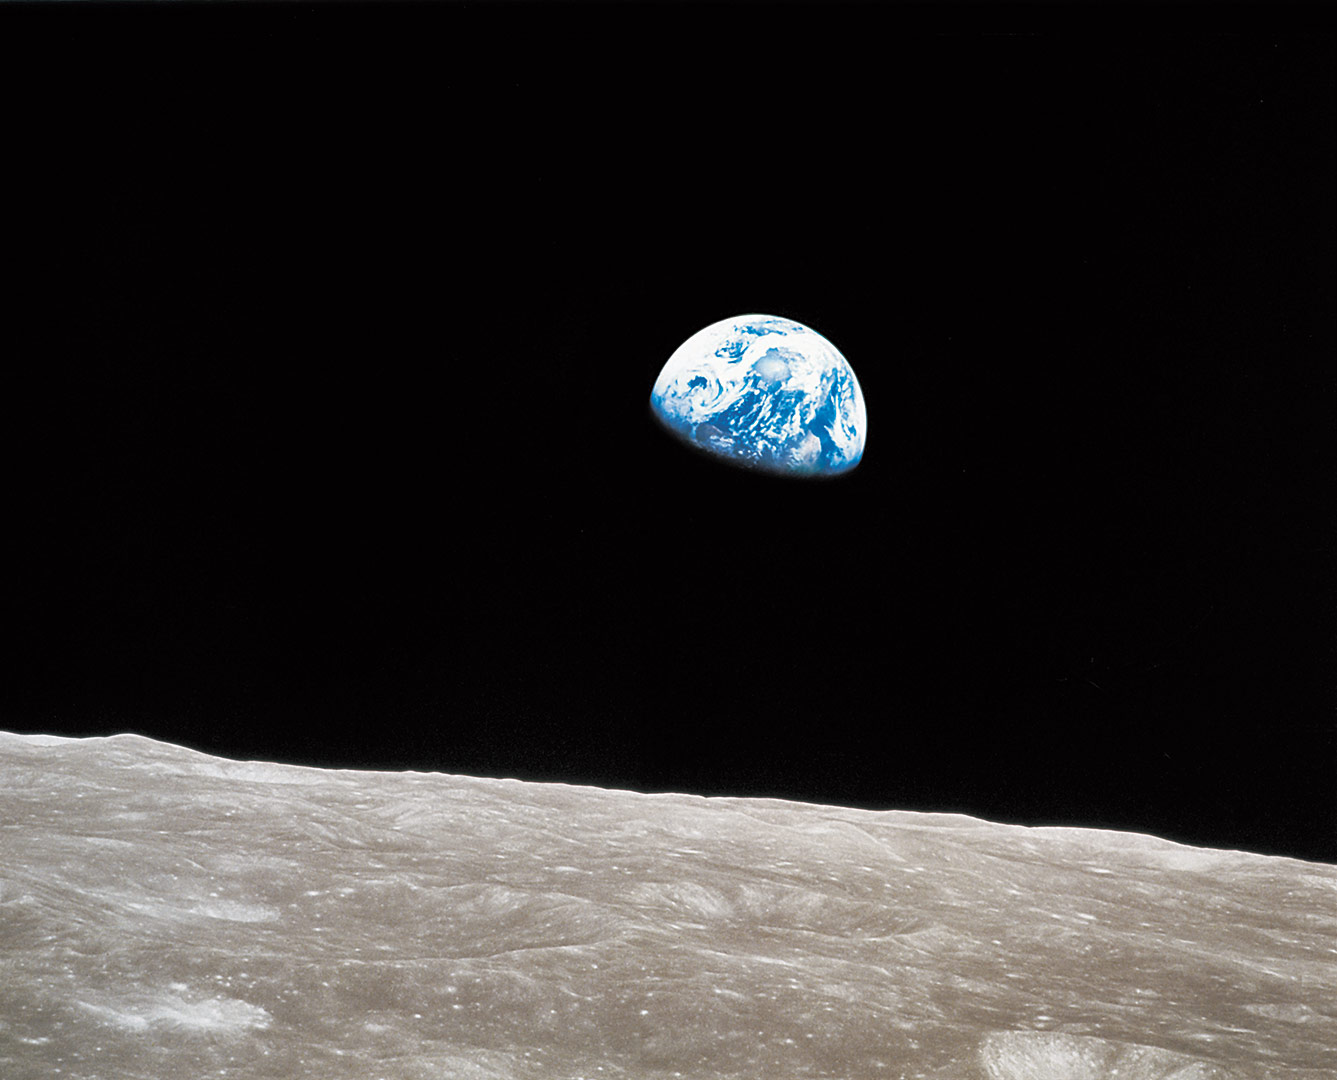
\includegraphics[width=0.9\linewidth]{earthrise.jpg}
  \end{wrapfigure}

  At the time that Apollo 8 launched, we were nearing the end of the set deadline
  for the Apollo program to reach the moon with nothing to show for it. After
  facing tremendous setbacks in the aftermath of the Apollo 1 disaster, the entire
  program had to reconsider how it would proceed and chose to do so in a safer and
  slower way, despite the ticking of the time clock. However, with only about a
  year to go, we managed to send, for the first time in the history of the known
  universe, a living being to another world. Not the surface per se, but orbiting
  the moon is still an achievement that the American public should be incredibly
  proud of.

  \section{ISS Expedition 16}

  \begin{center}
  \rowcolors{1}{lightgray}{white}
    \begin{tabular}{ >{\bfseries}r | p{3.5in} }
      \hline
      Launch Vehicle & Soyuz and Shuttle \\
      Crew & Peggy Whitson, 
             Yuri Malenchenko, 
             Clayton Anderson, 
             Daniel Tani,
             Leopold Eyharts, 
             Garrett Reisman \\
      Dates & 10 October 2007 - 19 April 2008 \\
      Mission Summary & Configuration of the Harmony Module, installation of
      Columbus and Kibo and arrival of the Jules Verne \\
      \hline
    \end{tabular}
  \end{center}

  Valentina Tereshkova often gets credit for being the first woman in space and,
  while this is true, I don't believe it to be quite the equality-seeking movve
  that it's often touted as. Not to diminish Tereshkova's flight by any means, but
  in the following 20 years only one other female cosmonaut flew in space.
  In fact, in that time, only one American female flew in
  space as well. 
 
  \begin{wrapfigure}{l}{0.25\textwidth}
    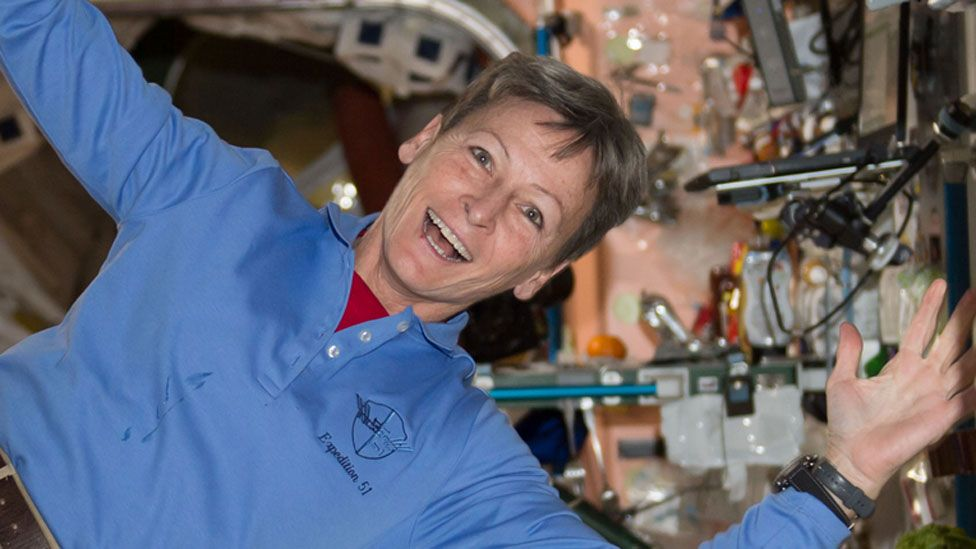
\includegraphics[width=0.9\linewidth]{whitson.jpg}
  \end{wrapfigure}

  It wasn't until the Shuttle era that we started to see female
  astronauts really achieve something closer to equality in human spaceflight,
  a field in which, biologically and physiologically speaking, they're actually
  quite a bit better suited for than men (women experience "space sickness" at
  rates far lower than men and also, in general, weigh less), meaning that the
  obstacles holding them back from equality in astronautics were necessarily
  socio-cultural.

  For my third most important mission I chose the mission in which Peggy Whitson
  became the first female ISS \textbf{\textit{commander}} an honor and responsibility that I
  believe required NASA to actually put themselves on the line and put their faith
  in a female astronaut, something that wasn't nearly as requisite when it comes 
  to simply putting women into space.


\end{document}
